\documentclass{article} % For LaTeX2e
\usepackage{iclr2018_conference,times}
\usepackage{hyperref}
\usepackage{url}
\usepackage{graphicx}
\usepackage{natbib}


\title{(tentative) Learning Neural Markers of Schizophrenia Disorder Using Recurrent Neural Networks}

% Authors must not appear in the submitted version. They should be hidden
% as long as the \iclrfinalcopy macro remains commented out below.
% Non-anonymous submissions will be rejected without review.

\author{Antiquus S.~Hippocampus, Natalia Cerebro \& Amelie P. Amygdale \thanks{ Use footnote for providing further information
about author (webpage, alternative address)---\emph{not} for acknowledging
funding agencies.  Funding acknowledgements go at the end of the paper.} \\
Department of Computer Science\\
Cranberry-Lemon University\\
Pittsburgh, PA 15213, USA \\
\texttt{\{hippo,brain,jen\}@cs.cranberry-lemon.edu} \\
\And
Ji Q. Ren \& Yevgeny LeNet \\
Department of Computational Neuroscience \\
University of the Witwatersrand \\
Joburg, South Africa \\
\texttt{\{robot,net\}@wits.ac.za} \\
\AND
Coauthor \\
Affiliation \\
Address \\
\texttt{email}
}

% The \author macro works with any number of authors. There are two commands
% used to separate the names and addresses of multiple authors: \And and \AND.
%
% Using \And between authors leaves it to \LaTeX{} to determine where to break
% the lines. Using \AND forces a linebreak at that point. So, if \LaTeX{}
% puts 3 of 4 authors names on the first line, and the last on the second
% line, try using \AND instead of \And before the third author name.

\newcommand{\fix}{\marginpar{FIX}}
\newcommand{\new}{\marginpar{NEW}}

%\iclrfinalcopy % Uncomment for camera-ready version, but NOT for submission.

\begin{document}


\maketitle

% Outline: 
% 1. Introduction: RNNs and CNNs being used for variety of recognition and diagnosis tasks. Problem with previous attempts
% to learn features from brain imaging data (fmri). High variability in brain responses across individuals.
% 2. Related Work: previous work on frmi, previous work to learn from videos, previous work to diagnose schizophrenia 
% 4. Methods
%   4.1 dataset
%   4.2 recurrent-convolutional neural nets for feature learning from fmri segments
% 5. Experiments: 
%   5.1 effectiveness of RNNs and R-CNNs to learn discriminative features from fmri
%	  5.2 generalizability of learned features across datasets
% 6. Discussion
% 7. Conclusion

\begin{abstract}
... Here we propose a new method based on recurrent-convolutional neural networks to automatically learn useful representations from short segments of fMRI recordings...
\end{abstract}

\section{Introduction}
*A key challenge in dealing with neuroimaging data comes from the inter- and intra-subject variability that any robust diagnosis system should be robust to. A prominent cause of these variabilities are due to small differences in the functional cortical mapping between individuals which calls for neural markers that are position and scale invariant.*

Diagnosis of psychiatric diseases can be a prolonged process. This is mainly due to lack of objective biological markers (such as the level of a metabolite in patient’s blood test) and similarity of symptoms among different diseases (e.g. depression phase of bipolar disorder and unipolar depression). Delayed and sometime inaccurate diagnosis results in belated less effective intervention. In addition, there is no objective biological marker for predicting treatment response in an individual. This oftentimes results in multiple changes in a patient’s prescription resulting in poor adherence given the medications side effects. Such inefficiency in diagnosis and treatment prognosis of psychiatric disorders is reflected in the global statistics [[burden of disease]] [[ as well as loca statistics]], with mental illness ranking first, before cancer and cardiac conditions, in terms of time lost to disability [WHO 2012 report] and costs \citep{Roehrig2016} [associated with the disease]. 

In recent years, machine learning techniques have shown success in identifying patients with mental or neurological disorders or predicting treatment response using brain imaging, especially structural and functional MRI (magnetic resonance imaging) data \citep{Gheiratmand2017, Orru2012, ?? Add more}. Almost all these studies extract features from imaging data and use the features in combination with standard classifiers, such as support vector machines (SVM) \citep{Orru2012, Wolfers2015} to discriminate between patients and controls or predict response to treatment [depression-new study]. (Less studies are available on the treatment response prediction, mainly due to lack of treatment response data, compared to diagnostics data) (Some typical imaging features extracted from fMRI or MRI include functional connectivity [], ALFF (amplitude of low-frequency fluctuations) [] for fMRI data, and voxel-based morphometry [], or gray matter thickness/volume [] for structural MRI. Such features may be extracted voxel-wise (where every voxel is a brain tissue of size ~1-33 mm3) or region-wise from predefined brain regions (such as thalamus, postcentral gyrus, etc.)

With deep learning techniques gaining outstanding performance in various fields including image classification [Refs], speech recognition [Refs], and video classification [Refs], among others, the approach is being recruited and explored in clinical applications, including those involving medical imaging data \citep{Shen2017, Litjens2017, Gulshan2016} [need comments on CNN? Re its vast use]. In addition to their potential to surpass the performance of other standard machine learning methods, deep learning methods are attractive because they can be directly applied to the data, skipping the need to extract hand-engineered features from the data – a step that is necessary in almost all other machine learning approaches [check statement correctness]. Deep Neural Networks might [or has the potential to] learn representations from brain images that might reveal useful information about abnormalities associated with the disease [check statement correctness]. 

Various deep learning methods have been employed in analysis of imaging data for various psychiatric and neurological disorders, including but not limited to Alzheimer’s disease (AD), ADHD, and Psychosis (see \citep{Vieira2017}). These methods include multi-layer perceptron (MLP), autoencoders (AE), deep belief networks, and convolutional neural networks citep[see][]{Vieira2017}[][for a review]. Most of these studies use structural MRI for predictions in neurological disorders, and much fewer studies use fMRI, which has been shown to be particularly relevant in predictive analysis of psychotic disorders (such as schizophrenia) (e.g. \citep{Damaraju2014, Calhoun2009}). fMRI data measures blood oxygen-level dependent signal (BOLD) at every brain voxel by taking a scan of the whole brain every 1-3 s. It can be thought of as a movie of the brain activity (reflected in BOLD signal – although the relationship between BOLD and neural activity is still under scrutiny [Ref-Amir Shmuel]), either in response to a task (e.g. a motor, sensory, or cognitive task) or simply at rest. 	

\citet{Plis14} showed that a restricted Boltzman machie (RBM) block \citep{Hinton2002} can extracted features from fMRI data, that are comparable to spatial and temporal maps extracted by ICA (independent component analysis) – one of the most commonly used methods to extract brain functional networks from fMRI data. They also showed that increasing the depth of a Deep Belief Network (DBN) \citep{Hinton06} (from 1 to 3), generated by stacking RBM blocks, applied to structural MRI data from patients with schizophrenia and healthy controls, results in features that discriminate more accurately between the two groups (from and F-score of 0.66 to 0.9, resp., in combination with an rbf-SVM). 
\citet{Suk2016} used a combination of a deep auto-encoder (DAE) and a hidden Markov Model (HMM) to discriminate between patients with mild cognitive impairment (MCI) and healthy controls. (They also modeled the dynamics of the functional connectivity networks in resting-state fMRI, assuming FC networks change over time and are not static.) First a DAE finds an embedding of the functional relations between brain regions (similar to \citep{Plis2014}), then a HMM estimates the dynamic characteristics of the functional networks in the embedded space for the MCI and control group separately. (During testing, the new sample is assigned to the group (MCI vs. HC) with the higher likelihood probability. \citet{Kim2016} used functional connectivity features, extracted from resting-state fMRI, in combination with a sparse autoencoder-based pretrained deep neural network (DNN), to discriminate between patients with schizophrenia and healthy controls. The DNN’s accuracy (85.5\%) surpassed the rbf SVM accuracy on the same dataset by 8.1\%. \citet{Sarraf2016} used 2-D convolutional neural network (CNN) to extract features from fMRI (and MRI) data for discriminating between patients with Alzheimer’s disease and healthy controls. In their approach, they decomposed each (resting-state) 4D fMRI data into a series of 2D images along z-axis (axial slices) and time and fed those as input to CNN architectures, LeNet \citep{LeCunn1998} and GoogleNet \citep{Szegedy2015} to train and test the adopted networks. (Authors achieved a very high classification accuracy of almost 100\% on the test set (as well as average over cross-validation folds), but it is not clear whether the set of subjects in the train and test sets, as well as cross-validation folds, are disjoint. This is extremely important, as we will also describe in our own work later in the Methods, to avoid “double-dipping”. If the samples from one subject appear in both train and test sets, there is no surprise the results are extremely good.) 

Here, our goal was to exploit both spatial and temporal information in the fMRI movie (at the whole-brain voxel-level) for identifying patients with schizophrenia. We propose using a recurrent convolutional neural network to exploit both spatial and temporal information in fMRI data. The proposed model involves a 3-D CNN followed by a sequential NN with LSTM units. The CNN extracts spatial features, which are fed to the LSTM model, which uses the dependencies between time points at every spatial location to generate an output {patient, control} (see Figure ??). To our knowledge, this is the first work to apply a recurrent CNN to fMRI data [for neurological/psychiatric diagnosis (here schizophrenia)]. As discussed earlier, most previous fMRI/machine learning studies, including some deep learning ones \citep{Kim2016}, use hand-crafted features, in particular functional connectivity features \citep{Gheiratmand2017}, which collapses the time dimension (of the BOLD signal) into one single number (i.e. the correlation coefficient between a pair of time-series). Such approach does not keep track of the relationships between spatial locations (e.g. voxel or brain regions) either. Here, we expand the work by \citet{Bashivan2015}, who successfully applied a recurrent CNN (with 2D convolutions) to EEG data in a mental load classification task, to fMRI data (using 3D convolutions). [[video classification idea]] We used fMRI data in response to an auditory oddball task and a working memory task from patients diagnosed with schizophrenia and healthy controls from FBIRN dataset [Ref]. The task is to predict a label {patient, control} based on the preprocessed fMRI BOLD signal per voxel. 

%%[[In the next sections, we will first describe ...]]
   
%%[[FBIRn data -- previously used with standard ML techniques and FC features [npj schz]]


\section{Related Work}

%MG: This is discussed in the Introduction. If not required by ICLR, no need for a separate section on related work.

\section{Methods}

\subsection{Dataset}
We used FBIRN phaseII fMRI dataset \citep{Keator2016}, downloaded from Function BIRN Data Repository, Project Accession Number 2007-BDR-6UHZ1 (fbirnbdr.nbirn.net:8080/BDR). It includes functional and structural data for patients with schizophrenia or schizoaffective disorder and age- and sex-matched healthy controls. We focused on two subsets of fMRI data acquired in response to two different tasks: 1) an Auditory Oddball (AO) task and 2) a working memory task (Sternberg Item Recognition Paradigm, SIRP). The fMRI data included whole-brain scans taken every 2s for a period of 280s and 360s for the AO and SIPR tasks respectively. There were 4 experiment runs (280s each) for the AO task and 3 runs for the SIRP task (360s each). 

A standard series of preprocessing stages was applied to each subject’s raw fMRI data using the FSL software package \citep{Jenkinson2002}. These included motion correction, tCompCor denoising, spatial filtering, high-pass temporal filtering, and linear registration to the MNI T1 template through subject’s T1 scan (see \citep[see]{Gheiratmand2017}[][for a more detailed description of the preprocessing stages]. The first 3 volumes in each run awere deleted for signal instability, resulting in a total of 137 volumes for the AO and 177 volumes for the SIRP task. Finally, a universal mask, i.e. the intersection of all subjects’ brains, was applied to each subject’s data, resulting in a common non-zero brain area comprising 26,949 voxels (brain tissue of size 3.4374 x 3.4375 x 5 mm).

After preprocessing and quality control, N = 95 subjects (46 patients, 49 controls) remained in the study (from a total of 164 subjects in both scanning sessions). (We used the data from the second scanning session, out of two, for no particular reason.)

\subsection{Recurrent-Convolutional Neural Networks}
We compared accuracy of recurrent neural networks (LSTM model) and recurrent-convolutional nerual networks (R-CNN) with baseline classifiers to learn discriminative features for the problem of distinguishing normal and schizophrenic individuals. We tried several different architectures consisting of LSTMs as well as R-CNNs. The input data was structured as a 3-dimensional tensor (3D brain scans). 

\textbf{Baseline Classifier}: We used a $L_1$-regularized logistic regression model and Support Vector Classifier (SVC) applied on voxel activations as the baseline models to compare against. Both of these models were trained on voxel values on all time-frames (did we do this??). 

\textbf{LSTM model}: All voxel values are reshaped into a vector and fed directly into a two-layer forward LSTM model. LSTMs are known for their ability in learning long-term dependencies between inputs. In this model the spatial relationship between voxels are ignored and LSTM learns the temporal relationship between activations in different voxels. 

\textbf{Conv-LSTM model}: 3-D activations for each time frame were fed into a 3D CNN. We used 3-dimensional convolutions followed by max-pooling to extract position and scale independent features that would generalize across individuals. Identical networks were used to process each time-frame with shared weights between them. Outputs of each CNN were then reshaped into a vector that was fed as input to the LSTM network at each time step. Figure-\ref{fig1} shows an overview of the recurrent-convolutional network used here. CNN part learns 3-D features that are invariant to translation and scaling and reduces the dimension of the input space before feeding it into LSTM. 

A batch size of 64 was used for all models. Larger convolutional models were trained synchronously on 16 GPUs. In both cases we experimented with varying number of time-frames included in each sample (i.e. 16 and 64).

\subsection{Training Details}
\label{training_details}
We used Adam optimizer with default parameter settings ($\beta_1=0.9, \beta_2=0.999, \epsilon=10^{-8}$). We included dropout in the input and outputs of the LSTM cells \citep{Zaremba2014} which contained most of the tunable parameters in our models. 

10-fold cross-validation was used to evaluate the performance for each proposed model. $l_2$ regularizer was used on all convolutional and fully connected weights. 
3D-convolutions of size $3\times3\times3$ with stride 1 were used. Each block of convolutions were followed by a maxpool layer of size 2 and stride 2. Feature map size was dividing by 2 after each maxpool layer. Size of the input to the network was $(53\times64\times37)$.

A different subset of subjects were assigned to the test set for each fold and data from the rest of the subjects were used for training and validation (without overlap between train and validation sets). For training, samples within each batch were generated by randomly selecting time windows from different subjects. All possible time windows of size $T$ from all subjects were used for training, validation and test. For each fold training was done for 10 folds. We used the validation set to for early stopping of training. After each training epoch, performance on the validation set was computed. Training was performed for 10 epochs and test performance was computed for the network state with highest validation score. 

** add figure on validation loss for RCNN

\begin{figure}[t]
\begin{center}
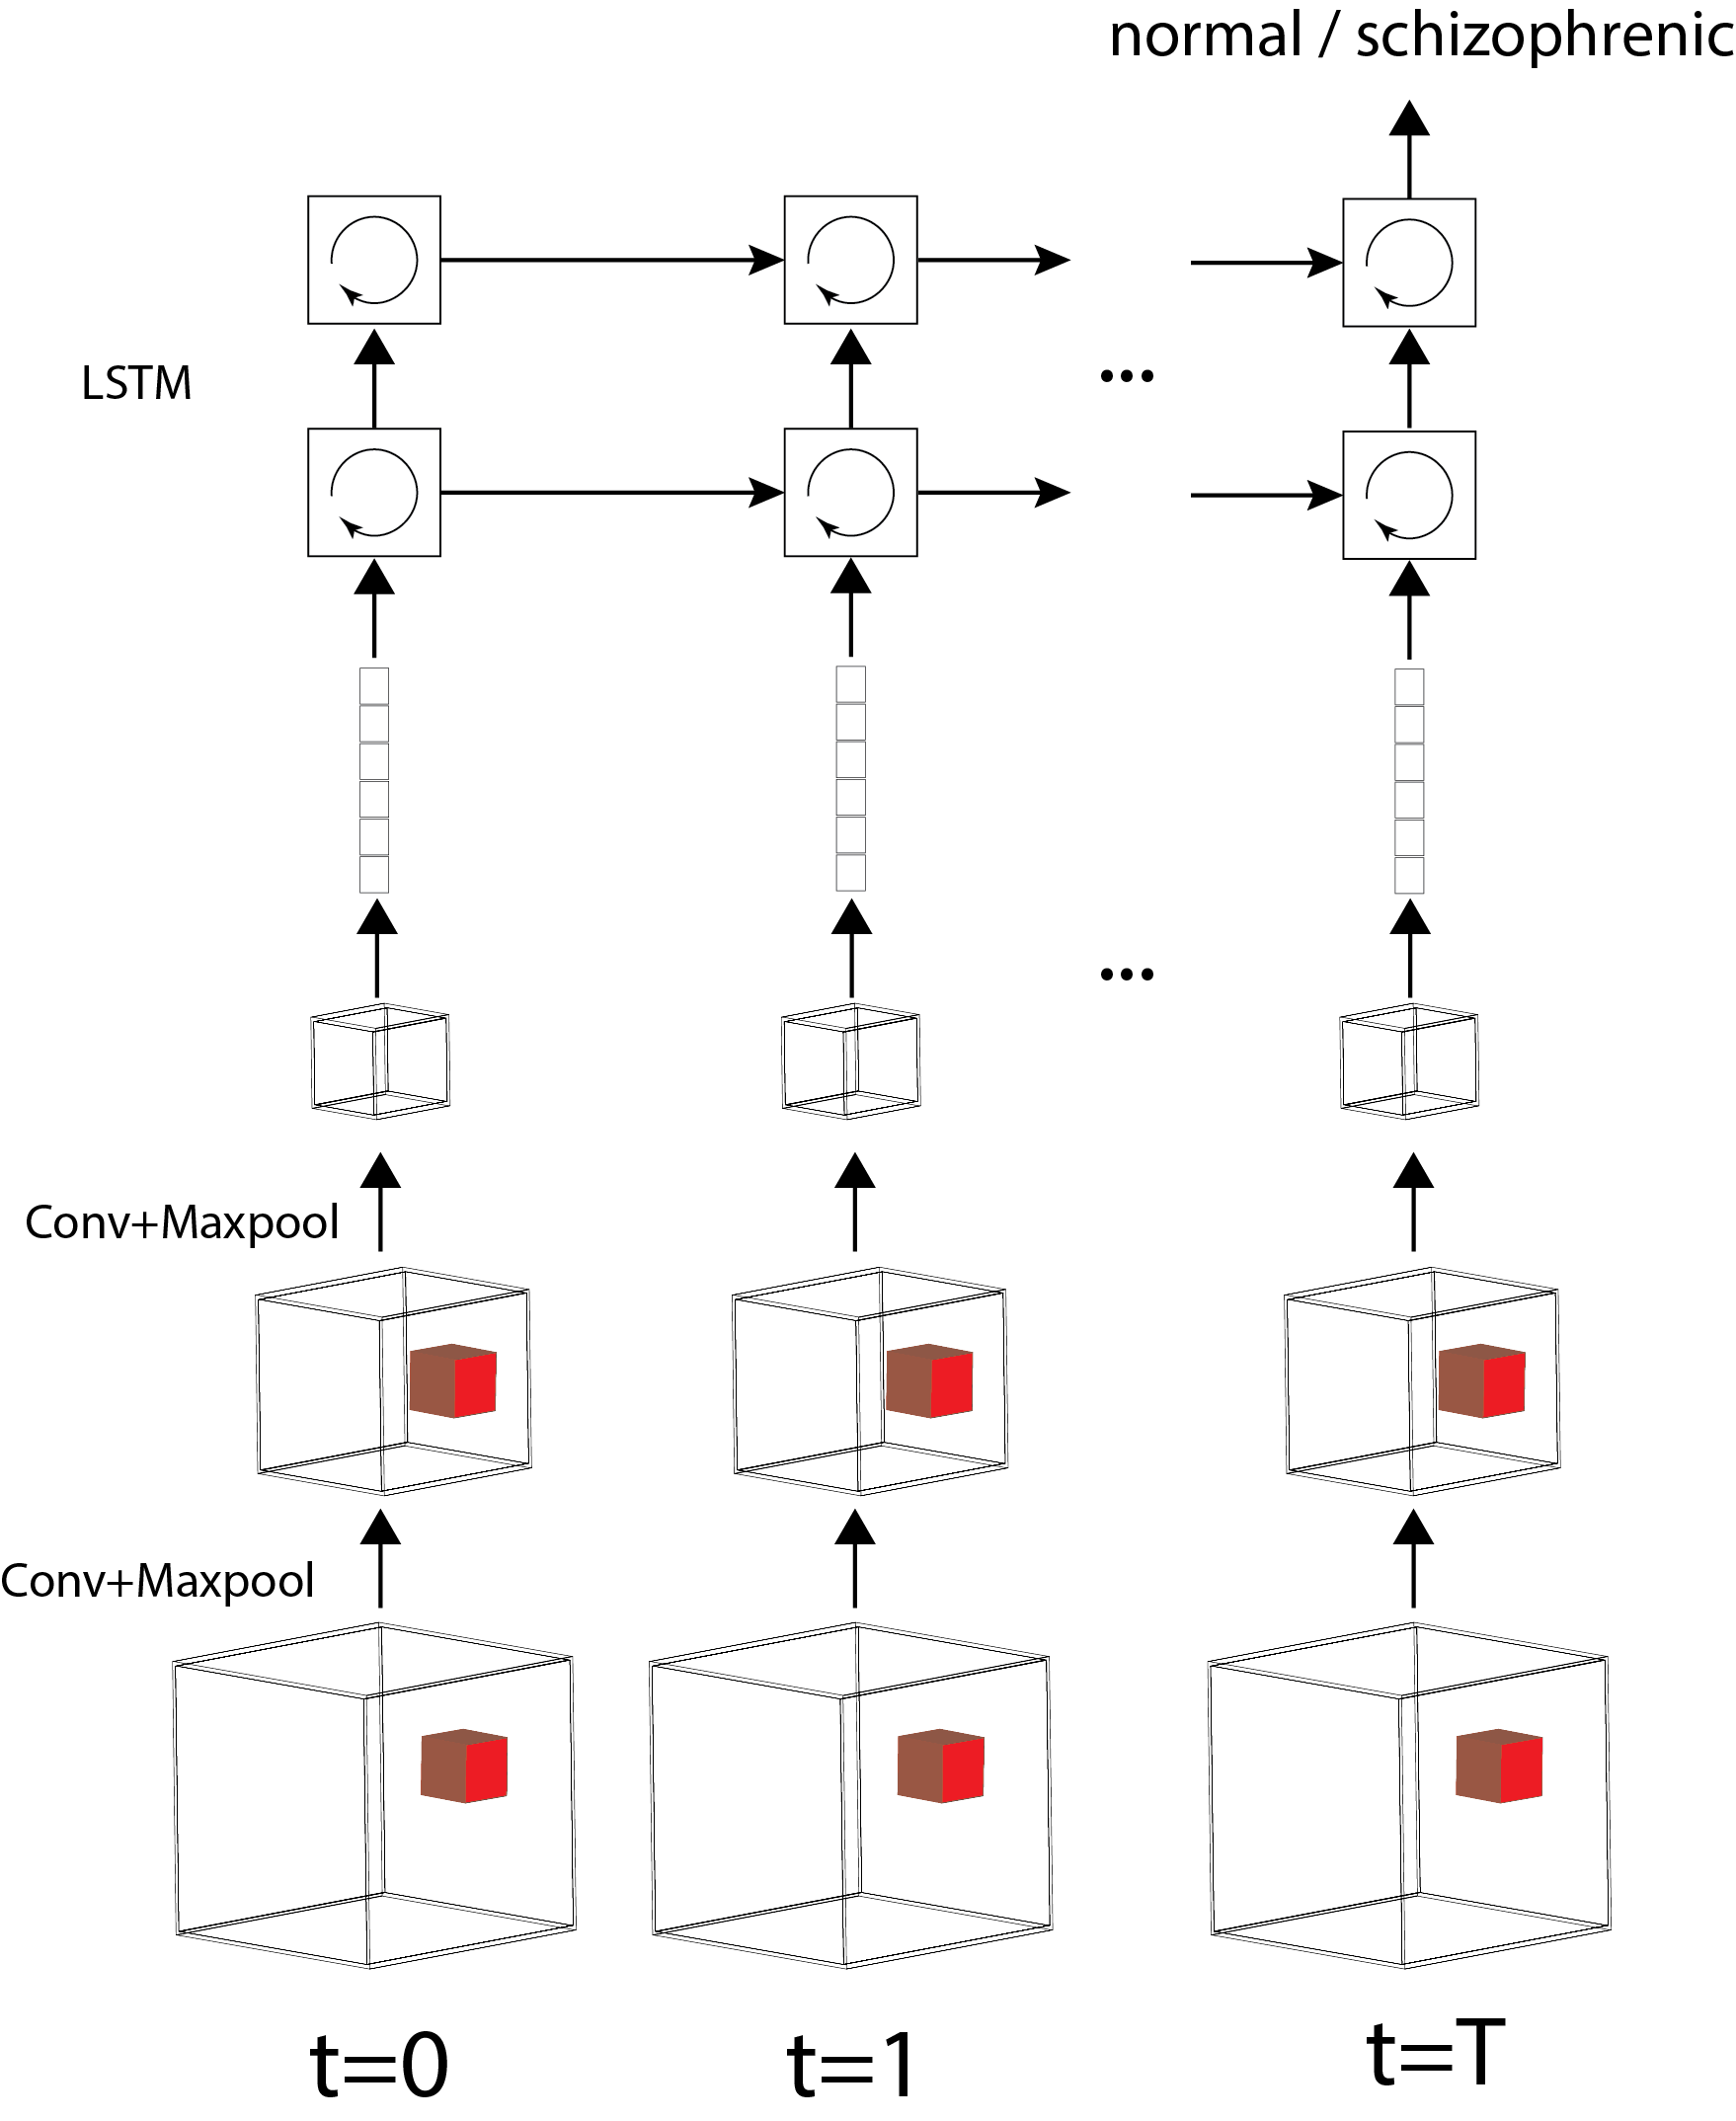
\includegraphics[width=3in]{figures/overview.png}
\end{center}
\caption{Overview of the method used.}
\label{fig1}
\end{figure}

\subsection{Data Preparation}
Preprocessed fMRI data was normalized in three steps: For each subject/run/voxel (i) the BOLD signal time-series was demeaned; (ii) The resulting time-series was divided by standard deviation (SD) of activation across the whole brain (all voxels and times). Next, each voxel’s time-series was standardized respective to the mean and SD of the voxel’s activation across all subjects and runs.  

Each fMRI sample (subject/run) was split into windows of 64 time points (or 128s) (i.e. a total of 137-63=74 samples for the AO and 114 for the SIRP task), which formed the input for training, evaluation, and testing of our models. A shorter time-frame of 16 volumes (32s) was also tested. Subjects in the training, evaluation, and test sets were disjoint, i.e. all samples corresponding to a subject were used only in one of the three above sets.  

\subsection*{Results}

We examined the performance of our models using two approaches. In the first approach, we compare the performance of LSTM and RCNN across various architectures and evaluate the model that yields the highest accuracy. In the second approach, we evaluated the robustness of our best models by training from the Auditory Oddball (AO) task and testing on a working memory task using the Sternberg Item Recognition Paradigm (SIRP). 

experimental setup: We performed all experiments on the XSEDE Xstream GPU cluster \citep{Towns2014} -- a petaFLOP Cray machine with 8 NVIDIA K80 card, 2 Intel Ivy-Bridge 10-core CPUs, and 256 GB of DRAM per node, with shared Lustre file system. 


\subsubsection*{LSTM and Recurrent Convolutional Neural Networks}

First we evaluate LSTM and recurrent convolutional neural network models using the configurations in table 1. We trained the models with the ??non-working AO task dataset. Table 2 shows the number of parameters used by each type of architecture, and the corresponding error achieved on the test set. 

The best recurrent convolutional model was obtained with architecture X containing two back-to-back convolutions in the first layer, one convolution in the second layer, and two back-to-back LSTMs in the third layer. We compared results using both 16 and 64 time-window samples while keeping the batch size fixed at 64 samples. For the model using 64 time windows, we noticed a significant improvement of 5\% in classification accuracy. 

Comparing the performance of the baseline model and deep learning, the test scores of LSTM and RCNN were 17.5\% better than linear SVM.  

In comparison to the best LSTM model, we noticed that LSTM scores slightly higher than RCNN. However, a closer examination reveals that RCNN exposed better training behavior across folds, with less fluctuation/variance in accuracy. ??In addition, most of the differences in accuracy can be attributed to the differences in subjects across sites. ??In particular, all folds from sites x,y,z achieve more than 66 \% accuracy while the remaining folds trained on data from site 6 showed little to no generalization or improvement over the baseline. [weren't the subjects shuffled before fold separation? Aren't the folds balanced as much as possible in terms of sites?]

\begin{figure}[t]
\begin{center}
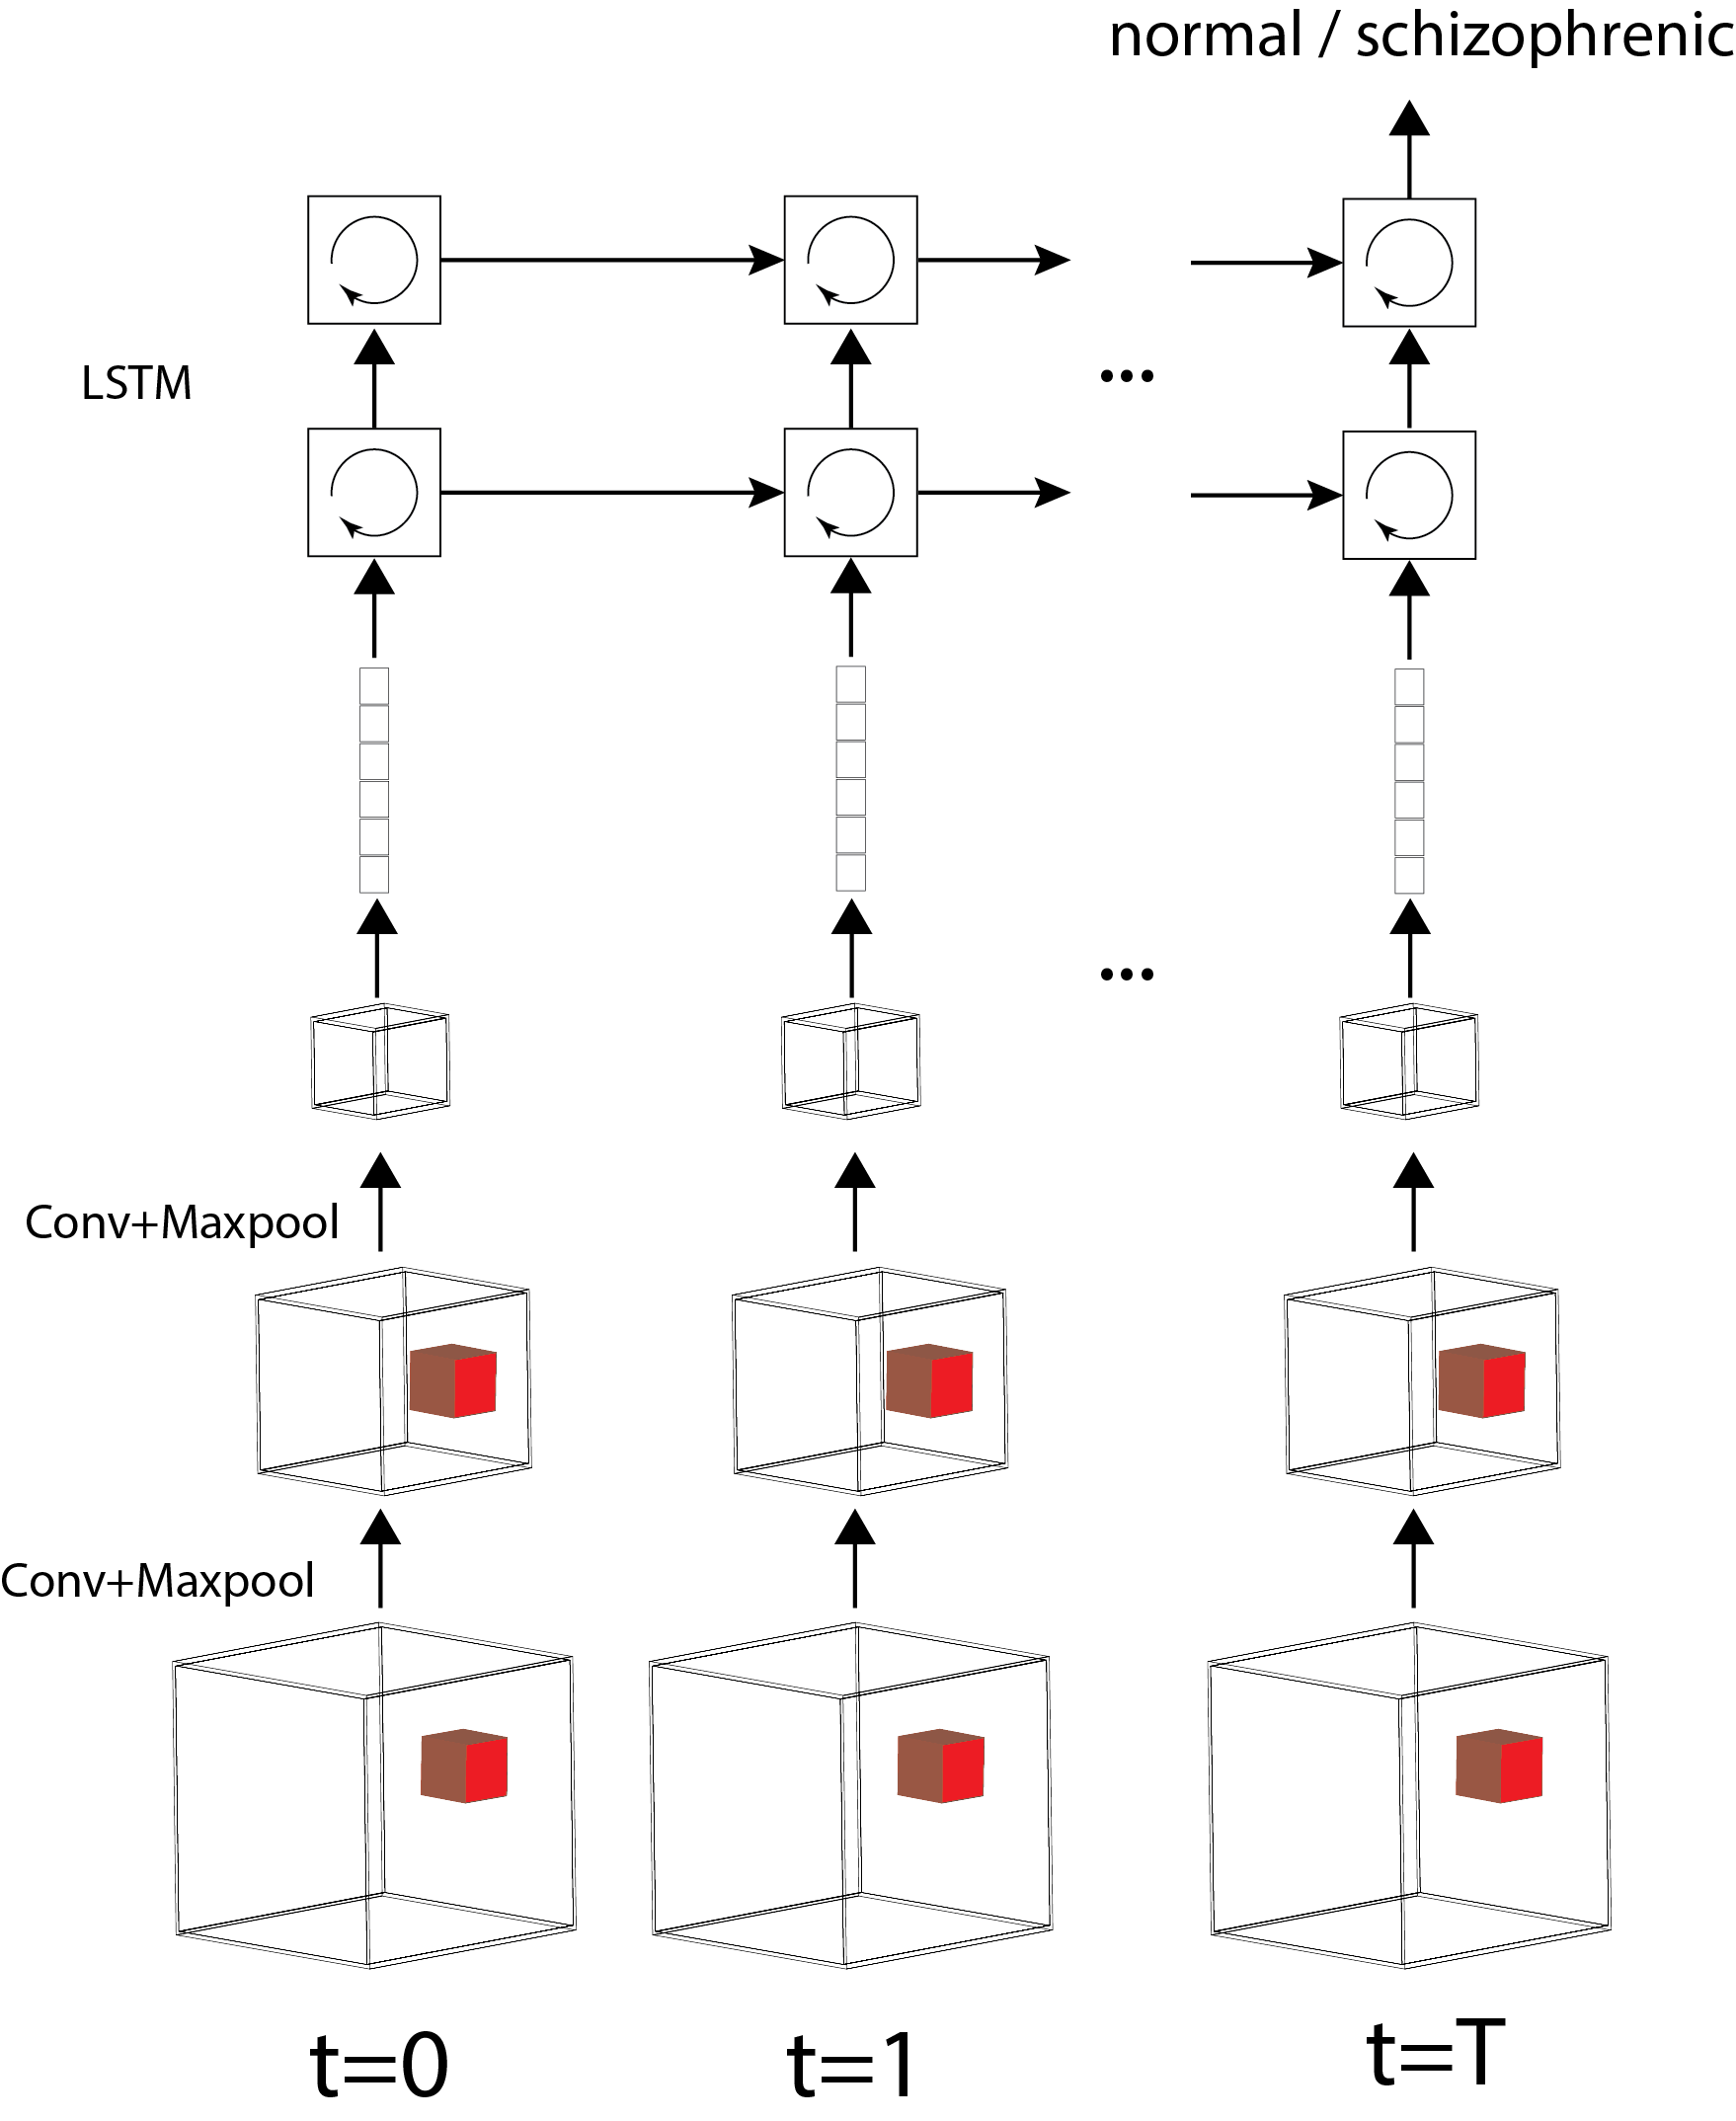
\includegraphics[width=3in]{figures/overview.png}
\end{center}
\caption{Overview of the method used.}
\label{fig1}
\end{figure}

\subsubsection*{Generalization across Datasets}

In order to see which model could generalize better across datasets, we compare the RCNN and LSTM models from approach 1 and trained each model using the AO dataset and then tested with the SIRP dataset. 

We found that the RCNN was invariant to the dataset and could generalize better than LSTM. (let us pray)

\subsubsection*{Acknowledgments}

Data used for this study were downloaded from the Function BIRN Data Repository (http://fbirnbdr.birncommunity.org:8080/BDR/), supported by grants to the Function BIRN (U24-RR021992) Testbed funded by the National Center for Research Resources at the National Institutes of Health, U.S.A.	
This work used the Extreme Science and Engineering Discovery Environment (XSEDE), which is supported by National Science Foundation grant number ACI-1548562, [and Compute Canada (www.computecanada.ca)??]. 
[[Also: "This work used the Extreme Science and Engineering Discovery Environment (XSEDE) resource-name at the service-provider through allocation allocationid."]]

Fundings: ? 


\bibliography{iclr2018_conference}
\bibliographystyle{iclr2018_conference}

\end{document}
